\documentclass[pre,reprint,superscriptaddress,longbibliography,amsmath,amssymb,floatfix]{revtex4-2}
\usepackage{graphicx}
\usepackage{bm}
\usepackage{xcolor}
\usepackage[colorlinks=true,linkcolor=blue,citecolor=blue,urlcolor=blue]{hyperref}

% Items only the author can confirm. Count must be zero at submission.
\newcommand{\human}[1]{\par\smallskip\noindent\fcolorbox{red!70!black}{yellow!12}{%
  \parbox{0.94\columnwidth}{\footnotesize\textbf{[AUTHOR]} #1}}\par\smallskip}

\newcommand{\Sv}{\mathbf{S}}
\newcommand{\nhat}{\hat{\mathbf n}}
\newcommand{\Tx}{T_\times}
\newcommand{\rx}{r_\times}
\newcommand{\TKT}{T_{\rm KT}}

\renewcommand{\topfraction}{0.95}
\renewcommand{\textfraction}{0.05}
\renewcommand{\floatpagefraction}{0.8}

\begin{document}

\title{Crossing Ising and Kosterlitz--Thouless lines in axis-locked tetrahedral spin bodies}

\author{Changyeon Won}
\email{cywon@khu.ac.kr}
\affiliation{Department of Physics, Kyung Hee University, Seoul 02447, Republic of Korea}

\date{\today}

\begin{abstract}
When an Ising and an XY order parameter are coupled, as in the fully frustrated XY model, the Ising and Kosterlitz--Thouless (KT) transitions can merge or stay apart, and how the two lines meet where their order reverses has been left open. We show that a uniaxial anisotropy turns a lattice of tetrahedral spin bodies---clusters of four antiferromagnetically bound classical spins---into this problem with a single tunable coupling: a quartic single-ion term locks a threefold body axis along the anisotropy axis, and the remaining variables are the time-reversal-odd sign $\sigma$ of the axial octupole and the time-reversal-even phase $\psi$ of the hexadecapole. The resulting XY--Ising model decouples exactly in two limits with opposite transition order, so the lines must cross; the lowest Ising--XY coupling operator is irrelevant there, which makes the crossing a decoupled tetracritical point, and a decoupling estimate with exact critical correlations predicts its position without free parameters. Pre-registered parallel-tempering Monte Carlo simulations up to $L=128$ place the crossing at $r_\times=4.340\pm0.024$ (prediction 4.31), find Ising ($\nu=1$) and KT scaling on both sides with no sign of a first-order merger, and resolve beyond it a window of hexadecapolar quasi-long-range order with short-ranged octupoles. In the full model of deformable bodies the effective description holds when the axis is stiff; its leading correction is a Debye--Waller reduction of each multipole coupling, weighted by $\frac12[l(l+1)-m^2]$ and caused only by relative tilts of neighboring bodies, which reproduces the full-model transition within 5\% for an axis-locking length of 0.77 lattice spacings but not for 4.5.
\end{abstract}

\maketitle

%=====================================================================
\section{Introduction}\label{sec:intro}
%=====================================================================

Many two-dimensional systems carry an Ising and an XY order parameter at once. The fully frustrated XY model of Josephson-junction arrays has a $\mathbb Z_2$ chirality and a $U(1)$ phase~\cite{TeitelJayaprakash1983,Korshunov2006}; multiband superconductors that break time reversal combine a $\mathbb Z_2$ with a superconducting phase~\cite{Bojesen2014}; coupled nematic and hexatic orders lock into discrete states~\cite{DrouinTouchette2022}. The minimal lattice description is the general XY--Ising model of Granato, Kosterlitz, Lee, and Nightingale~\cite{GKLN1991,LGK1991},
\begin{equation}
H=-\sum_{\langle ab\rangle}\big[(A+B\sigma_a\sigma_b)\cos\Delta\psi+C\sigma_a\sigma_b\big],
\label{eq:GKLN}
\end{equation}
with $\sigma_a=\pm1$ and $\Delta\psi=\psi_a-\psi_b$; the line $A=B$ contains the fully frustrated XY model. Its phase diagram contains a phase with Ising order and a disordered phase angle, a phase with quasi-long-range XY order and disordered Ising variables, and the fully ordered and fully disordered phases~\cite{LGK1991,Berge1986,NGK1995,Ma2024}. Depending on the couplings, the two transitions either occur separately, in either order, or merge into a single line whose nature has been debated for decades~\cite{LGK1991,NGK1995,HPV2005,Korshunov2006}.

A basic question about this phase diagram has received little attention: where the Ising transition stops lying above the KT transition and starts lying below it, \emph{how do the two lines meet}? They could join a merged line, end at a multicritical point with new exponents, or simply cross. The lines in Ref.~\cite{LGK1991} are drawn from Monte Carlo data and the decoupling analysis of Yosefin and Domany~\cite{YosefinDomany1985} gives estimates of each line, but neither settles the junction. Part of the reason is that physical realizations rarely allow one to tune through the reversal with a single parameter.

\human{Novelty claim. Please confirm that neither Refs.~\cite{LGK1991,YosefinDomany1985} nor later work (Refs.~\cite{NGK1995,HPV2005,Ma2024}) resolves how the Ising and KT lines join at the reversal point. The paragraph above says ``has received little attention'' and ``neither settles the junction''.}

Here we show that such a realization arises naturally from \emph{spin bodies}, the clusters of $n$ classical spins introduced in Ref.~\cite{PaperI}. For $n=4$ the intra-body exchange holds the spins at the corners of a regular tetrahedron, and the inter-body exchange couples the bodies through their octupole ($l=3$) and hexadecapole ($l=4$) moments. Adding a uniaxial single-ion anisotropy has two consequences that we derive exactly. First, because the tetrahedron is a spherical 2-design~\cite{Delsarte1977}, the quadratic anisotropy has no first-order effect, and the axis selection is controlled by one coefficient $\Gamma$ that combines the quartic anisotropy with the deformability of the body. Second, when a threefold ($C_3$) axis is selected, the bodies reduce exactly to Eq.~\eqref{eq:GKLN} with $\sigma$ the sign of the axial octupole, odd under time reversal, and $\psi$ the phase of the in-plane hexadecapole, even under time reversal. The ratio $C/B=5/4$ is fixed by geometry, while $A/B$ is set by the ratio of quartic to cubic inter-body exchange and can be tuned from zero.

Our main results are as follows.
(i)~The two limits $A=0$ and $B=0$ of this model are exactly decoupled and have opposite orders of transitions, so the Ising and KT lines must cross in between. Combining the decoupling argument of Ref.~\cite{YosefinDomany1985} with the exact nearest-neighbor correlations at the Ising and KT critical points predicts the crossing at $r_\times=A/B=4.31$ without free parameters.
(ii)~At the crossing the lowest coupling between the Ising energy density and the XY gradient has scaling dimension 3 and is irrelevant, so the crossing is a decoupled tetracritical point in the sense of Kosterlitz, Nelson, and Fisher~\cite{KNF1976}.
(iii)~Monte Carlo simulations with decision rules fixed in advance confirm the crossing at $r_\times=4.340\pm0.001\,({\rm stat})\pm0.024\,({\rm sys})$, separate Ising and KT scaling on both sides, and an inverted window in which the time-reversal-even hexadecapole has quasi-long-range order while the octupole is short ranged.
(iv)~In the full model of deformable bodies, tilts of the locked axis reduce the couplings by Debye--Waller factors that depend on the multipole channel as $\frac12[l(l+1)-m^2]$ and only through relative tilts; this correction accounts for the full-model transition when the axis is stiff on the lattice scale.

The paper is organized as follows. Section~\ref{sec:model} defines the model and its symmetry. Section~\ref{sec:selection} derives the axis selection. Section~\ref{sec:eff} derives the effective model, its decoupled limits, and the crossing. Section~\ref{sec:mc} presents the simulations of the effective model and Sec.~\ref{sec:full} those of the full model. Section~\ref{sec:disc} discusses realizations and open questions.

%=====================================================================
\section{Model and symmetry}\label{sec:model}
%=====================================================================

Each site $a$ of a square lattice ($z=4$) hosts four unit vectors $\Sv_{a,i}$. Following Ref.~\cite{PaperI} we take
\begin{align}
H_0&=\sum_a\sum_{i<j}\big[Jx^{aa}_{ij}+K(x^{aa}_{ij})^2\big]\nonumber\\
&\quad-\sum_{\langle ab\rangle}\sum_{i,j=1}^{4}\big[G(x^{ab}_{ij})^3+H_4(x^{ab}_{ij})^4\big],
\label{eq:H0}
\end{align}
with $x^{ab}_{ij}=\Sv_{a,i}\cdot\Sv_{b,j}$ and $J=1$. The antiferromagnetic intra-body terms favor a regular tetrahedron; the inter-body terms are ferromagnetic and do not distinguish the spins of a body. We add a single-ion anisotropy
\begin{equation}
V=\sum_a\sum_{i=1}^4\big[a_2P_2(\hat z\cdot\Sv_{a,i})+a_4P_4(\hat z\cdot\Sv_{a,i})\big],
\label{eq:V}
\end{equation}
where $a_2=2D/3$ for $D(S^z)^2$ and $a_4=8B_4/35$ for $B_4(S^z)^4$. Expanding all pair functions in Legendre channels gives the spectrum $\kappa_l=f_l-zg_l$ of Ref.~\cite{PaperI},
\begin{align}
\kappa_1&=J-\tfrac35zG, & \kappa_2&=\tfrac23K-\tfrac47zH_4,\nonumber\\
\kappa_3&=-\tfrac25zG, & \kappa_4&=-\tfrac{8}{35}zH_4 .
\label{eq:kappa}
\end{align}
Because $V$ is a sum of single-body terms, the uniform-state theorem of Ref.~\cite{PaperI} still holds: at zero temperature all bodies take the same shape and orientation, and the problem reduces to one body in the pair potential $\Phi(x)=\sum_l\kappa_lP_l(x)$ plus $V$.

The anisotropy reduces the symmetry from $O(3)$ to $O(2)\times\mathbb Z_2^{\mathcal T}$. A tetrahedral body has three twofold rotoreflection ($S_4$) axes and four threefold ($C_3$) axes. If an $S_4$ axis is locked along $\hat z$, the residual stabilizer is $D_{2d}$ and the order-parameter manifold is $U(1)/\mathbb Z_2$; if a $C_3$ axis is locked, the stabilizer is $C_{3v}$ and the manifold is $\mathbb Z_2\times U(1)/\mathbb Z_3$. The $\mathbb Z_2$ in the latter case distinguishes bodies whose apex points up or down [Fig.~\ref{fig:model}(b)]; time reversal maps one onto the other. Both manifolds have trivial $\pi_2$, and the non-Abelian defects of the isotropic tetrahedral phase~\cite{PaperI,Mermin1979} are confined by the anisotropy into string-like objects of width
\begin{equation}
\ell_\Gamma=\sqrt{\rho/|\Gamma|},
\label{eq:lGamma}
\end{equation}
where $\rho$ is the orientational stiffness of the bodies and $\Gamma$ the axis-locking energy defined next. This length controls the validity of the effective model (Sec.~\ref{sec:full}).

\begin{figure}[!tbp]
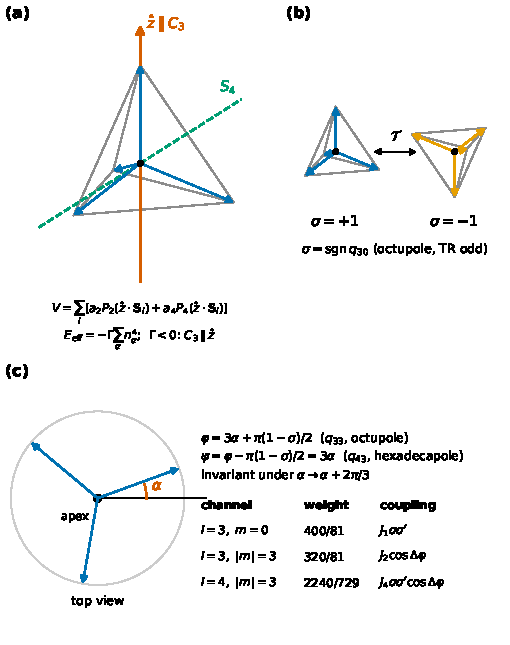
\includegraphics[width=\columnwidth]{fig/fig1_model.pdf}
\caption{A tetrahedral spin body under uniaxial anisotropy keeps one body axis along $\hat z$, and its remaining state is an Ising octupole sign $\sigma$ and an XY hexadecapole phase $\psi$. (a)~Spin body with the $C_3$ axis along $\hat z$ (selected for $\Gamma<0$) and one $S_4$ axis. (b)~$\sigma=\operatorname{sgn}q_{30}$; time reversal $\mathcal T$ inverts the body, so $\sigma$ is odd under $\mathcal T$. (c)~Top view: $\varphi=3\alpha+\pi(1-\sigma)/2$ is the phase of the octupole component $q_{33}$ and $\psi=3\alpha$ that of the hexadecapole component $q_{43}$; the multipole weights of the three channels that couple neighbors and the couplings they produce [Eq.~\eqref{eq:C3}].}
\label{fig:model}
\end{figure}

%=====================================================================
\section{Axis selection}\label{sec:selection}
%=====================================================================

\paragraph*{First order.} The four vertices of a regular tetrahedron form a spherical 2-design, $\sum_i(\hat z\cdot\Sv_i)^2=4/3$ for every orientation. The $a_2$ term in Eq.~\eqref{eq:V} therefore does not depend on orientation at first order. The $a_4$ term is the $l=4$ cubic harmonic,
\begin{equation}
E^{(1)}=a_4\Big(\frac73-\frac{35}{9}K_n\Big),\qquad K_n\equiv\sum_{\alpha}n_\alpha^4 ,
\label{eq:E1}
\end{equation}
where $\nhat$ is $\hat z$ expressed in the cube frame of the body; $K_n=1$ for an $S_4$ axis and $K_n=1/3$ for a $C_3$ axis along $\hat z$.

\paragraph*{Second order.} Without a first-order torque the $a_2$ force acts only on the deformation modes of the body, which under $T_d$ split into $E$ and $T_2$. At an $S_4$ orientation the force lies entirely in $E$, $|f_E|^2=8a_2^2$; at a $C_3$ orientation entirely in $T_2$, $|f_{T_2}|^2=8a_2^2/3$. Relaxing the body against the stiffnesses $\lambda_E=\frac83\Phi''(-\frac13)$ and $\lambda_{T_2}=\frac89[3\Phi'(-\frac13)+2\Phi''(-\frac13)]$ of Ref.~\cite{PaperI} gives a second-order energy that is again linear in $K_n$ (Appendix~\ref{app:gamma}). Together,
\begin{equation}
E_{\rm eff}(\nhat)=-\Gamma K_n,\qquad
\Gamma=\frac{35}{9}a_4+2a_2^2\Big(\frac{3}{\lambda_E}-\frac{1}{\lambda_{T_2}}\Big).
\label{eq:Gamma}
\end{equation}
$\Gamma>0$ selects an $S_4$ axis along $\hat z$ and $\Gamma<0$ a $C_3$ axis, independently of the sign of $D$. The stiffnesses already contain the inter-body couplings through $\kappa_l$, so Eq.~\eqref{eq:Gamma} is the axis-locking energy per body of the whole lattice at zero temperature.

Figure~\ref{fig:selection}(a) compares Eq.~\eqref{eq:Gamma} with direct minimization of a single body at fixed orientation: the relaxed energy is linear in $K_n$ over all orientations. The deviation from the formula is proportional to the anisotropy amplitude and changes sign with $a_2$ [Fig.~\ref{fig:selection}(c)], as expected for the next order ($a_4^2$, $a_2^3$).

\paragraph*{Which axis.} The sign of the $a_2^2$ term is set by
\begin{align}
3\lambda_{T_2}-\lambda_E&=\tfrac{8}{27}(27\kappa_1-63\kappa_3+35\kappa_4)\nonumber\\
&=\tfrac{8}{27}(27J+9zG-8zH_4),
\label{eq:criterion}
\end{align}
in which $\kappa_2$, and with it the intra-body biquadratic exchange $K$, cancels. Throughout the tetrahedral (T) ground state this combination is positive [Fig.~\ref{fig:selection}(b)]: the T phase ends at a competing square-planar state (two orthogonal antiparallel pairs, energy $E_{\rm Sq}-E_{\rm T}=2\kappa_2-\frac{40}{9}\kappa_3+\frac{185}{54}\kappa_4$) before $8zH_4$ can exceed $27J+9zG$. Hence the common quadratic anisotropy alone always selects $S_4$, and a $C_3$ axis requires a quartic anisotropy $a_4<0$ with $|a_4|>\frac{18}{35}a_2^2(3/\lambda_E-1/\lambda_{T_2})$.

\human{The T--Sq boundary $zH_4=0.692K+0.923zG$ also cuts into the $K=0.5$ plane of Ref.~\cite{PaperI} as a thin wedge. Decide whether to mention this here (it bears on Paper~I) or keep only the $K=2$ boundary used in this work.}

\paragraph*{The $S_4$ branch.} For completeness, an $S_4$ axis along $\hat z$ leaves the in-plane angle $\alpha$ with a twofold degeneracy, and with $\theta=2\alpha$ the bodies form the generalized XY model
\begin{equation}
H_{S_4}=-\sum_{\langle ab\rangle}\Big[\frac{32}{9}G\cos\Delta\theta+\frac{32}{81}H_4\cos2\Delta\theta\Big],
\end{equation}
with time reversal acting as $\theta\to\theta+\pi$. Its half-vortex phase~\cite{LeeGrinstein1985,Poderoso2011,Canova2016} would be a time-reversal-even hexadecapolar phase, but it needs $H_4/G$ of order 20, which lies outside the T phase. We do not pursue this branch.

\begin{figure}[!tbp]
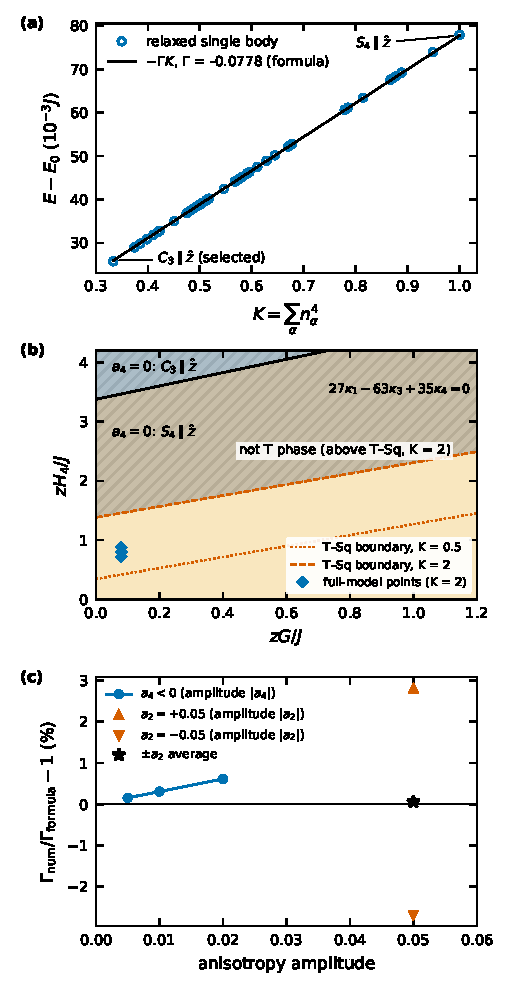
\includegraphics[width=\columnwidth]{fig/fig2_axis_selection.pdf}
\caption{The anisotropy selects the body axis through one cubic coefficient $\Gamma$, which the second-order formula~\eqref{eq:Gamma} gives to within 0.6\%, and within the T phase a $C_3$ axis requires $a_4<0$. (a)~Relaxed single-body energy at fixed orientation versus $K_n=\sum_\alpha n_\alpha^4$ (43 orientations, $a_4=-0.02$, $J=1$, $K=2$, $zG=0.08$, $zH_4=0.80$): a line of slope $-\Gamma$. (b)~Selection by $a_2$ alone, Eq.~\eqref{eq:criterion}; the boundary $27J+9zG-8zH_4=0$ lies above the T--Sq boundary, so in the T phase $a_2$ always selects $S_4$. Grey hatching: above the T--Sq boundary at $K=2$ the ground state is not tetrahedral. Diamonds: parameters of the full-model simulations of Sec.~\ref{sec:full}. (c)~Relative deviation of the numerical $\Gamma$ from Eq.~\eqref{eq:Gamma}; it is linear in the amplitude (next order), and the $\pm a_2$ average agrees to 0.06\%.}
\label{fig:selection}
\end{figure}

%=====================================================================
\section{Effective model of the $C_3$ phase}\label{sec:eff}
%=====================================================================

\paragraph*{Couplings from multipole weights.} For a rigid tetrahedron only the $l=3$ and $l=4$ channels couple neighboring bodies, since the $l=1,2$ multipoles of a 2-design vanish. The bond energy is $-g_l\frac{4\pi}{2l+1}{\rm Re}\,\mathbf q^{(l)}_a\cdot\mathbf q^{(l)*}_b$ with $g_3=\frac25G$, $g_4=\frac{8}{35}H_4$ and $q^{(l)}_m=\sum_iY_{lm}(\Sv_i)$. With a $C_3$ axis along $\hat z$ the nonzero components are $q_{30}$ and $q_{3,\pm3}$ for $l=3$ and $q_{40}$ and $q_{4,\pm3}$ for $l=4$ (Appendix~\ref{app:weights}). Let $\alpha$ be the in-plane angle of the body and $\sigma=\operatorname{sgn}q_{30}=\pm1$. Then $q_{33}\propto e^{i\varphi}$ with $\varphi=3\alpha+\pi(1-\sigma)/2$, while $q_{43}\propto e^{i\psi}$ with $\psi=3\alpha$. Inserting the weights gives
\begin{equation}
H_{C_3}=-\sum_{\langle ab\rangle}\big[J_1\sigma_a\sigma_b+(J_4+J_2\sigma_a\sigma_b)\cos(\psi_a-\psi_b)\big],
\label{eq:C3}
\end{equation}
\begin{equation}
J_1=\frac{160}{81}G,\qquad J_2=\frac{128}{81}G,\qquad J_4=\frac{512}{729}H_4 ,
\label{eq:J}
\end{equation}
up to a constant. Equation~\eqref{eq:C3} is Eq.~\eqref{eq:GKLN} with $(A,B,C)=(J_4,J_2,J_1)$. The geometry fixes $J_1/J_2=5/4$; the only free ratio is
\begin{equation}
r\equiv\frac{J_4}{J_2}=\frac49\,\frac{zH_4}{zG}.
\label{eq:r}
\end{equation}
In the octupole frame, $\cos(\varphi_a-\varphi_b)=\sigma_a\sigma_b\cos(\psi_a-\psi_b)$ and the same Hamiltonian reads $-\sum[J_1\sigma\sigma'+(J_2+J_4\sigma\sigma')\cos\Delta\varphi]$. Time reversal flips $\sigma$ and shifts $\varphi$ by $\pi$ but leaves $\psi$ unchanged: $\sigma$ and $e^{i\varphi}$ are octupolar (odd), $e^{i\psi}$ is hexadecapolar (even). The orientational stiffness is isotropic by Schur's lemma, $\rho=\frac{128}{9}G+\frac{512}{81}H_4$, the same for both axes.

\paragraph*{Two exactly decoupled limits.} For $J_4=0$ ($H_4=0$), $\sigma$ and $\varphi$ decouple exactly: the octupole channel cannot mix $\sigma\sigma'$ with $\cos\Delta\varphi$. The time-reversal-odd sign orders first, at the Onsager temperature~\cite{Onsager1944} $T_I=2.269J_1$, and $\varphi$ follows at the KT temperature~\cite{KosterlitzThouless1973,Hasenbusch2005} $T_{\rm KT}=0.893J_2$. For $J_2=0$ ($G=0$), $\sigma$ and $\psi$ decouple exactly, and the time-reversal-even phase $\psi$ orders by itself at $0.893J_4$, above any Ising transition once $r$ is large. The two limits have opposite orders of transitions. Since both lines are continuous in $r$, they must cross at some $r_\times$.

\paragraph*{Where they cross.} Near each line one variable is critical and the other enters through a bond average. In the $\psi$ frame the Ising variable sees the coupling $J_1+J_2\langle\cos\Delta\psi\rangle$, and in the region where $\sigma$ is correlated the phase sees $J_4+J_2\langle\sigma\sigma'\rangle$, so~\cite{YosefinDomany1985}
\begin{align}
T_I&\simeq2.269\big(J_1+J_2\langle\cos\Delta\psi\rangle\big),\nonumber\\
T_{\rm KT}&\simeq0.893\big(J_4+J_2\langle\sigma\sigma'\rangle\big).
\label{eq:decoupling}
\end{align}
At a crossing both variables are critical, and the averages take their exact critical values: $\langle\sigma\sigma'\rangle=1/\sqrt2$ for the square-lattice Ising model at $T_c$~\cite{Onsager1944}, and $\langle\cos\Delta\psi\rangle=0.723$ for the XY model at $T_{\rm KT}$. This gives, with no adjustable parameter,
\begin{align}
T_\times&=2.269(J_1+0.723J_2)=7.07\,G,\nonumber\\
r_\times&=\frac{T_\times}{0.893J_2}-\frac{1}{\sqrt2}=4.31 .
\label{eq:rx}
\end{align}
Equation~\eqref{eq:decoupling} is an approximation away from the crossing; only Eq.~\eqref{eq:rx} uses it where its inputs are exact. The value 0.723 is from our own simulations of the XY model at $T_{\rm KT}$.

\human{The value $\langle\cos\Delta\psi\rangle=0.723$ at $T_{\rm KT}$ comes from our Wolff simulations, not from a published table. If a literature value (e.g., from Ref.~\cite{Hasenbusch2005}) is available, cite it here.}

\paragraph*{Why they cross rather than merge.} At the crossing the fixed point is the product of the Ising and KT fixed points. The lowest coupling allowed by the $\mathbb Z_2\times U(1)$ symmetry is $\varepsilon_\sigma(\nabla\psi)^2$, the Ising energy density times the XY gradient energy. Its scaling dimension is $1+2=3>2$, so it is irrelevant with eigenvalue $y=-1$; the product of $\varepsilon_\sigma$ with the vortex fugacity, of dimension 2 at $T_{\rm KT}$, is irrelevant for the same reason. The crossing is therefore a decoupled tetracritical point~\cite{KNF1976}: four phases meet, and each line keeps its own universality class through the crossing. The lines are not smooth there. The KT temperature depends on $\langle\sigma\sigma'\rangle$, which has the $t\ln|t|$ singularity of the Ising energy, so the KT line inherits a weak kink at $r_\times$.

\paragraph*{Domain walls and fractional vortices.} An Ising wall can keep either $\psi$ or $\varphi$ continuous. The first costs $2(J_1+J_2)$ per bond and the second $2(J_1+J_4)$. For $r<1$ the cheaper wall has $\psi$ jumping by $\pi$, so a wall that ends must end on a $\pi/3$ vortex of the body angle $\alpha$, as in the fully frustrated XY model~\cite{Korshunov2006}. Near $r_\times\approx4.3$ the cheaper wall keeps $\psi$ continuous and binds no vortex, consistent with decoupling.

%=====================================================================
\section{Monte Carlo of the effective model}\label{sec:mc}
%=====================================================================

\paragraph*{Method.} We simulate Eq.~\eqref{eq:C3} with the rigid couplings~\eqref{eq:J} ($G=1$) on $L\times L$ square lattices with periodic boundaries, $L=32$--128. Each sweep combines Metropolis updates, a Wolff cluster for $\varphi$~\cite{Wolff1989}, and two cluster moves that flip $(\sigma,\varphi)\to(-\sigma,\varphi+\pi)$. The first holds $\varphi$ fixed and has bonds $J_1+J_4\cos\Delta\varphi$, which are frustrated for $r\gtrsim1$. The second holds $\psi$ fixed and has bonds $J_1+J_2\cos\Delta\psi\ge J_1-J_2=32G/81>0$, which are never frustrated because $J_1/J_2=5/4$. Without the second move the Ising autocorrelation time at $L=64$ was 190--1500 sweeps; with it, $\tau_{\rm int}\le3.4$ sweeps for all runs. Replica exchange (parallel tempering)~\cite{HukushimaNemoto1996} uses temperature ladders designed for an exchange acceptance of at least 0.2 per attempt between every neighboring pair. The number of clusters per sweep is tuned in the first half of equilibration and then frozen; a state-dependent stopping rule biases the ensemble (Appendix~\ref{app:numerics}). Each run has $10^3$ equilibration and $2\times10^4$ measurement sweeps.

All decision rules, including the criteria for a crossing, for decoupled tetracritical behavior, and for a first-order merger, were written down before the production runs. A run is accepted only if quarter-split averages agree, $\tau_{\rm int}\le n_{\rm meas}/200$ for every temperature and observable, there are at least 20 complete round trips of the replicas, and every exchange acceptance is at least 0.2; random and ordered starts agree on both sides of the crossing. All 57 production runs passed. Observables are combined by multiple-histogram reweighting~\cite{FerrenbergSwendsen1989} with jackknife errors~\cite{MadrasSokal1988}.

The Ising temperature $T_I$ is the $L\to\infty$ extrapolation of Binder-cumulant crossings~\cite{Binder1981} of $\sigma$ (shift $\propto L^{-1/\nu-\omega}$, $\nu=1$, $\omega=1.75$). The KT temperature is the temperature at which the helicity modulus $\Upsilon_\psi$ of all sizes best fits the Weber--Minnhagen form~\cite{WeberMinnhagen1988}
\begin{equation}
\frac{\pi\Upsilon_\psi(L)}{2T}=1+\frac{1}{2\ln L+C}.
\label{eq:WM}
\end{equation}
For the pure XY model the same procedure with $L\le64$ gives $T_{\rm KT}=0.8906$ against the accepted 0.8929~\cite{Hasenbusch2005}, a bias of $-0.25\%$; we carry it as a systematic error and apply it in the direction that weakens each decision.

\begin{figure}[!tbp]
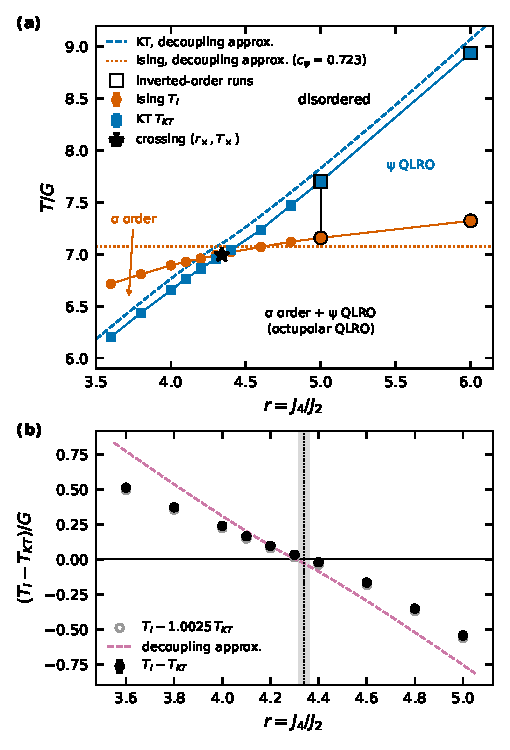
\includegraphics[width=\columnwidth]{fig/fig3_phase_diagram.pdf}
\caption{The Ising and KT lines of the $C_3$ effective model cross at $r_\times=4.340(1)(24)$, $T_\times=6.995(1)(7)\,G$, and beyond the crossing their order is inverted. (a)~$T$--$r$ phase diagram: $T_I$ (Binder crossings, $L\to\infty$) and $T_{\rm KT}$ (Weber--Minnhagen) for $r=3.6$--5.0 and 6.0 (open frames: runs testing the inverted order), joined by thin lines; decoupling approximations~\eqref{eq:decoupling} for the KT line (dashed) and the Ising line (dotted, evaluated with the critical value $\langle\cos\Delta\psi\rangle=0.723$ and valid near the crossing only); star: crossing. Labels give the four phases. (b)~$T_I-T_{\rm KT}$ versus $r$; open circles use $1.0025\,T_{\rm KT}$ (Weber--Minnhagen bias bound); grey band: systematic uncertainty of $r_\times$; dashed: decoupling approximation.}
\label{fig:phase}
\end{figure}

\paragraph*{The crossing.} Table~\ref{tab:TT} and Fig.~\ref{fig:phase} show the result. For $r\le4.0$ the Ising transition lies above the KT transition by more than 70 standard errors, and for $r\ge4.6$ below it by more than 50; the difference changes sign between $r=4.3$ ($+0.033\pm0.002$) and $r=4.4$ ($-0.021\pm0.002$). A straight-line fit of $T_I-T_{\rm KT}$ over all $r$, the estimator fixed in advance, gives
\begin{align}
r_\times&=4.340\pm0.001\pm0.024,\nonumber\\
T_\times&=(6.995\pm0.001\pm0.007)\,G,
\label{eq:rxmc}
\end{align}
where the second error is the shift obtained by raising all $T_{\rm KT}$ by the Weber--Minnhagen bias. The fit has $\chi^2/{\rm dof}=526/8$ because $T_I-T_{\rm KT}$ bends toward smaller slope near the crossing, so its statistical error does not capture the model error; linear interpolation between $r=4.3$ and 4.4, which assumes least, gives $r_\times=4.361\pm0.003\pm0.033$ and $T_\times=(7.008\pm0.010)\,G$. Both agree with the prediction $r_\times=4.31$ within the systematic error. The predicted $T_\times=7.07\,G$ is 1\% high, so the decoupling estimate locates the crossing in $r$ better than in $T$. The bending of $T_I-T_{\rm KT}$ is consistent with the $t\ln|t|$ kink of the KT line, but our data do not resolve it.

\begin{table}[!tbp]
\caption{Transition temperatures of the $C_3$ effective model (units of $G$). $T_I$: Binder crossings extrapolated to $L\to\infty$; $T_{\rm KT}$: Weber--Minnhagen fit over $L=32$--96 (to 128 for $r=4.0$--4.6). Errors are combined jackknife errors including the covariance of $T_I$ and $T_{\rm KT}$ from shared runs; $T_{\rm KT}$ carries an additional systematic $-0.25\%$ (see text).}
\label{tab:TT}
\begin{ruledtabular}
\begin{tabular}{cccc}
$r$ & $T_I$ & $T_{\rm KT}$ & $T_I-T_{\rm KT}$\\
\colrule
3.6 & 6.7161(17) & 6.2031(66) & 0.5130(67)\\
3.8 & 6.8072(17) & 6.4355(31) & 0.3717(35)\\
4.0 & 6.8932(8)  & 6.6533(22) & 0.2399(21)\\
4.1 & 6.9284(10) & 6.7629(20) & 0.1655(23)\\
4.2 & 6.9585(8)  & 6.8620(22) & 0.0965(24)\\
4.3 & 6.9902(9)  & 6.9573(16) & 0.0329(18)\\
4.4 & 7.0197(9)  & 7.0404(17) & $-0.0207(19)$\\
4.6 & 7.0706(10) & 7.2363(26) & $-0.1657(29)$\\
4.8 & 7.1203(18) & 7.4715(36) & $-0.3512(42)$\\
5.0 & 7.1579(21) & 7.7019(38) & $-0.5440(43)$\\
6.0 & 7.3225(18) & 8.9403(54) & $-1.6178(55)$\\
\end{tabular}
\end{ruledtabular}
\end{table}

\paragraph*{Decoupled tetracritical behavior.} On both sides of the crossing, at $r=4.2$ and 4.4, each transition keeps its own scaling (Fig.~\ref{fig:collapse}). The Binder cumulant of $\sigma$ collapses on $(T-T_I)L$ with $\nu=1$ for all sizes and both $r$; separate fits give $\nu=1.023\pm0.017$ and $1.004\pm0.015$ and crossing values $U^*=0.61$--0.62, the Ising values. The helicity modulus at $T_{\rm KT}$ follows the Weber--Minnhagen form~\eqref{eq:WM} with slope 1. Independently of the fit, the ratio $\xi_\psi/L$ at $T_{\rm KT}$ agrees with the pure XY model at the same $L$ within 0.005 for all $r$. The specific-heat maximum grows as $\ln L$ (fit $p$-values 0.43 and 0.31), and an $L^2$ growth is rejected ($p\sim10^{-48}$ and $10^{-36}$). Energy histograms are single peaked for every $r$ and $L$, and $C_{\max}/L^2$ decreases with $L$ everywhere. We find no sign of a first-order merger.

\begin{figure}[!tbp]
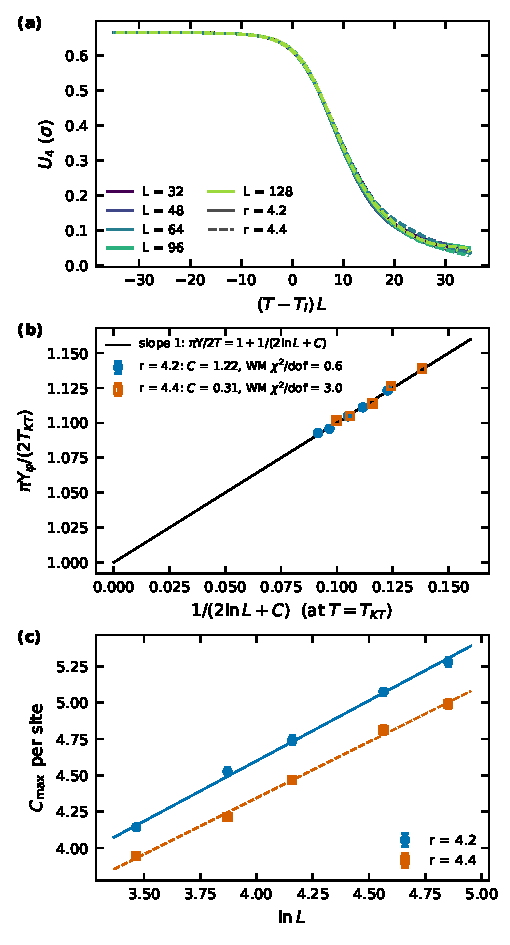
\includegraphics[width=\columnwidth]{fig/fig4_crossing_collapse.pdf}
\caption{On both sides of the crossing ($r=4.2$, 4.4) the Ising and KT transitions keep their own scaling, as expected for a decoupled tetracritical point. (a)~Binder cumulant of $\sigma$ versus $(T-T_I)L$ ($\nu=1$): all sizes and both $r$ on one curve. (b)~At $T=T_{\rm KT}$, $\pi\Upsilon_\psi/(2T)$ versus $1/(2\ln L+C)$ lies on the slope-1 line of Eq.~\eqref{eq:WM} for $L=32$--128 ($C=1.22$ and 0.31 fitted with the slope fixed). Because $T_{\rm KT}$ is itself the Weber--Minnhagen fit ($\chi^2/{\rm dof}=0.6$ and 3.0), this panel shows the quality of that fit rather than an independent test. (c)~The specific-heat maximum grows as $\ln L$ (lines: fits, $p=0.43$ and 0.31); $L^2$ growth is rejected.}
\label{fig:collapse}
\end{figure}

\paragraph*{The inverted window.} Beyond the crossing the hexadecapole orders before the octupole sign. At $r=6.0$ the window $T_I=7.322(2)<T<T_{\rm KT}=8.940(5)\,G$ satisfies all criteria fixed in advance at three temperatures inside it: the Binder cumulant of $\sigma$ decreases toward zero with $L$, $\Upsilon_\psi>2T/\pi$, the decay exponent of $\psi$ is $\eta_\psi=0.16$--0.20, below the KT bound 1/4, and the octupole phase $\varphi$ decays exponentially (effective $\eta_\varphi\approx2$, i.e., an $L$-independent susceptibility). In this window the system has quasi-long-range order of a time-reversal-even quantity, $e^{3i\alpha}$, while every time-reversal-odd quantity is short ranged. At $r=5.0$ the window $7.159(2)<T<7.699(4)\,G$ is present with the same exponents ($\eta_\psi=0.19$--0.22), but one criterion fails at the lowest test temperature, $0.135\,G$ above $T_I$: the Binder cumulant drops from $L=32$ to 96 by a factor 0.526, short of the required 1/2. The $\sigma$ correlation length there saturates at $\xi_\sigma\approx26$, so $L=96$ is only $3.8\,\xi_\sigma$; we attribute the failure to finite size but did not run larger lattices.

%=====================================================================
\section{Beyond the axis-locked limit}\label{sec:full}
%=====================================================================

The effective model assumes rigid bodies with the axis exactly along $\hat z$. In the full model~\eqref{eq:H0}+\eqref{eq:V} bodies deform and their axes tilt. Deformation renormalizes the couplings at the few-percent level: relaxing two bodies at $K=2$ gives $r_{\rm eff}\approx0.94\,r$ and $J_1/J_2\approx1.155$, which by Eq.~\eqref{eq:decoupling} moves the crossing to $r_\times\approx4.07$. Tilts have a larger effect.

\paragraph*{Full-model simulations.} We simulated the full model with the local moves of Ref.~\cite{PaperI} and parallel tempering at $J=1$, $K=2$, $a_2=0$, $a_4=-0.02$ ($\Gamma=-0.078$), on lattices $L=16$--32. With $zG=0.08$ and $zH_4=0.72$, 0.80, 0.88 the relaxed couplings give $r_{\rm eff}=3.68$, 4.05, 4.42, on both sides of the relaxed crossing. Each body is mapped onto the effective variables through its multipoles in the laboratory frame ($\sigma\leftarrow q_{30}$, $e^{i\varphi}\leftarrow q_{33}$, $e^{i\psi}\leftarrow q_{43}$), and $T^{\rm full}_\Upsilon$ is the temperature at which the twist stiffness of the body angle reaches the KT value at $L=24$. These runs do not meet our equilibration criteria ($\tau_{\rm int}=300$--1800 sweeps); we quote as error half the spread between random and ordered starts and grade the full-model conclusions below as indicative. The transition is about 40\% lower than in the effective model with the same relaxed couplings, far outside that spread, and the axis is not locked: $\langle K_n\rangle=0.42$ below and 0.52 above the transition, compared with 1/3 for a locked $C_3$ axis and 0.6 for random orientations.

The deficit decreases as the axis becomes stiffer. Scaling the inter-body couplings by $s$, $(zG,zH_4)=s\,(0.08,0.80)$, at fixed $a_4$ reduces the locking length~\eqref{eq:lGamma} from $\ell_\Gamma=4.46$ ($s=1$) to 0.77 ($s=0.03$), and the ratio $R=T^{\rm full}_\Upsilon/T_{\rm eff}$ rises monotonically from 0.60 to 0.87 (Table~\ref{tab:full}, Fig.~\ref{fig:dw}).

\paragraph*{Debye--Waller factors of multipole couplings.} Tilting a body by a small angle $\theta$ about an axis perpendicular to $\hat z$ multiplies the $(l,m)$ component of its multipole by the Wigner function $d^l_{mm}(\theta)=1-\frac14[l(l+1)-m^2]\theta^2+O(\theta^4)$; the leakage into $m\pm1$ is first order in $\theta$ but averages out of the bond product. If the two bodies of a bond tilt independently, the coupling in channel $(l,m)$ is reduced by
\begin{equation}
\frac{J^R_{lm}}{J_{lm}}=1-\tfrac12\big[l(l+1)-m^2\big]\langle\theta^2\rangle ,
\label{eq:DW}
\end{equation}
with coefficients 6 for $J_1$ $(3,0)$, 1.5 for $J_2$ $(3,3)$, and 5.5 for $J_4$ $(4,3)$. Within one $l$, the axial component $m=0$ is the most sensitive [coefficient $l(l+1)/2$] and the in-plane component $|m|=l$ the least (coefficient $l/2$). Tilt fluctuations therefore weaken the octupole-sign coupling $J_1$ and the hexadecapole coupling $J_4$ much more than $J_2$: they lower both $J_1/J_2$ and $r$, and so shift the crossing to larger bare $r$.

Rotation invariance makes the correction depend only on relative tilts. The bond depends on the relative rotation $R_a^{-1}R_b$, whose Euler decomposition gives $D^l_{mm}=e^{-im(\alpha+\gamma)}d^l_{mm}(\beta_{ab})$, where $\alpha+\gamma$ is the relative twist, already contained in $\cos\Delta\psi$, and $\beta_{ab}$ is the angle between the two $C_3$ axes. The exact reduction is therefore $\langle d^l_{mm}(\beta_{ab})\rangle$, a common tilt of the two bodies costs nothing, and at linear order Eq.~\eqref{eq:DW} becomes $1-\frac12[l(l+1)-m^2]\langle\theta^2\rangle(1-C_{nn})$ with $C_{nn}=\langle\bm\theta_a\cdot\bm\theta_b\rangle/\langle\theta^2\rangle$.

\begin{table}[!tbp]
\caption{Full spin-body model versus the effective model ($J=1$, $K=2$, $a_4=-0.02$, $(zG,zH_4)=s(0.08,0.80)$, $L=24$). $\ell_\Gamma$: locking length~\eqref{eq:lGamma}; $\langle\theta^2\rangle$, $C_{nn}$: measured tilt of the $C_3$ axis and its nearest-neighbor correlation at $T^{\rm full}_\Upsilon$. $R=T^{\rm full}_\Upsilon/T_{\rm eff}$ with bare relaxed couplings, with the per-body factor~\eqref{eq:DW}, and with the exact relative-tilt average $\langle d^l_{mm}(\beta_{ab})\rangle$. Errors: half the spread of random and ordered starts (full model not equilibrated by our criteria).}
\label{tab:full}
\begin{ruledtabular}
\begin{tabular}{cccccccc}
$s$ & $\ell_\Gamma$ & $\Gamma/T_{\rm eff}$ & $\langle\theta^2\rangle$ & $C_{nn}$ & $R_{\rm bare}$ & $R_{\rm body}$ & $R_{\rm rel}$\\
\colrule
1    & 4.46 & $-0.56$ & 0.097 & 0.32 & 0.603(1) & 1.094(2) & 0.801(2)\\
0.3  & 2.44 & $-1.84$ & --    & --   & 0.692(2) & --       & --      \\
0.1  & 1.41 & $-5.51$ & --    & --   & 0.773(8) & --       & --      \\
0.03 & 0.77 & $-18.3$ & 0.026 & 0.10 & 0.87(4)  & 0.99(4)  & 0.97(4) \\
\end{tabular}
\end{ruledtabular}
\end{table}

\paragraph*{Test.} We measured the tilt of each body's $C_3$ axis directly, inserted it into Eq.~\eqref{eq:DW} and into the exact relative average, and simulated the effective model with the reduced couplings. The decision rule, fixed in advance, required $|R-1|\le0.05$ at both $s=1$ and $s=0.03$. It is not met (Table~\ref{tab:full}). At $s=0.03$ ($\ell_\Gamma=0.77$, $6\langle\theta^2\rangle\approx0.16$) both prescriptions bring $R$ within 5\% of 1: $0.99\pm0.04$ per body and $0.97\pm0.04$ with relative tilts. At $s=1$ ($\ell_\Gamma=4.5$) the per-body factor, which ignores the neighbor correlation $C_{nn}=0.32$, overcorrects ($R=1.09$), and the relative average undercorrects ($R=0.80$). The relative tilt distribution itself is well described: $\langle\beta^2_{ab}\rangle\approx2\langle\theta^2\rangle(1-C_{nn})$ [Fig.~\ref{fig:dw}(b)], but 8\% of bonds have $\beta_{ab}>35^\circ$, where the small-angle picture and even the identification of a body axis break down.

We conclude that the Debye--Waller reduction of the couplings by tilt fluctuations is the main cause of the deficit, and that the linear factor reproduces the full model within 5\% when the largest reduction, $6\langle\theta^2\rangle$ for $J_1$, is below about 0.2. The relative-tilt average leaves a 20\% difference at $s=1$, which points to effects beyond the bond average, such as body deformation and axis defects. One such effect is that tilt fluctuations make the couplings fluctuate; at second order in the cumulant expansion this lowers the stiffness further, in the direction of the remaining deficit, by an amount we estimate at about 10\%.

\begin{figure}[!tbp]
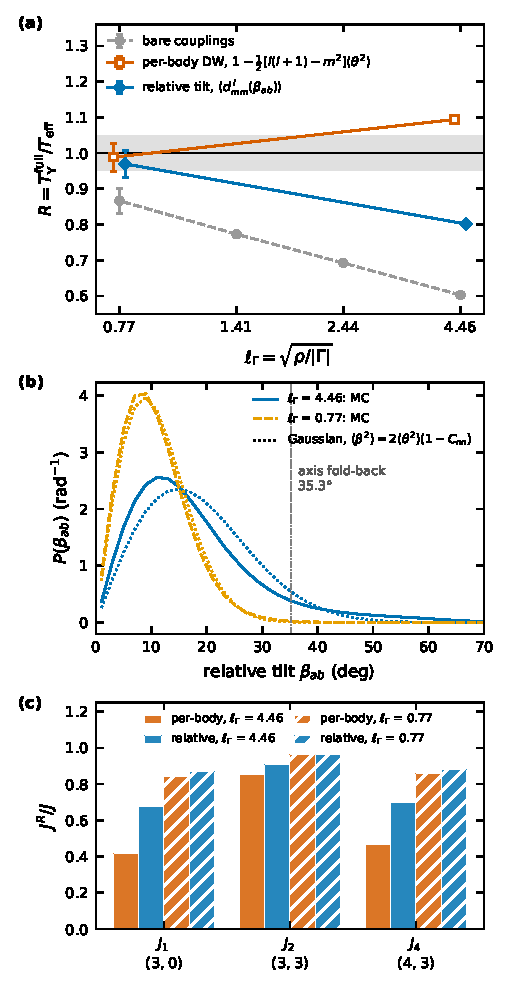
\includegraphics[width=\columnwidth]{fig/fig5_debye_waller.pdf}
\caption{The effective model with Debye--Waller-reduced couplings reproduces the full spin-body model at $\ell_\Gamma=0.77$ (central values within 5\%), while at $\ell_\Gamma=4.5$ the per-body and relative-tilt prescriptions bracket it. (a)~$R=T^{\rm full}_\Upsilon/T_{\rm eff}$ versus $\ell_\Gamma$: bare couplings, per-body factor~\eqref{eq:DW} with the measured tilt, and exact bond average $\langle d^l_{mm}(\beta_{ab})\rangle$; grey band: $\pm5\%$. (b)~Distribution of the relative tilt $\beta_{ab}$ at $T^{\rm full}_\Upsilon$, with the Gaussian of variance $2\langle\theta^2\rangle(1-C_{nn})$; above $35.3^\circ$ a tilted axis is closer to another $C_3$ axis of the body. (c)~Reduction factors $J^R/J$ per channel $(l,|m|)$: the axial channel $J_1$ and the hexadecapole $J_4$ are reduced most.}
\label{fig:dw}
\end{figure}

%=====================================================================
\section{Discussion}\label{sec:disc}
%=====================================================================

\paragraph*{What is new.} The four phases of the general XY--Ising model~\cite{LGK1991}, the existence of an XY-ordered phase with disordered Ising variables~\cite{Berge1986,Ma2024}, and the decoupling method~\cite{YosefinDomany1985} are known. Our contribution is the junction of the two lines: an exact argument that they cross, a parameter-free estimate of where, an irrelevance argument that makes the crossing a decoupled tetracritical point, and a numerical confirmation with errors. The spin bodies add a microscopic realization in which the Ising and XY variables are identified as the sign of an octupole and the phase of a hexadecapole, $C/B=5/4$ is fixed by geometry, and $A/B$ is tuned by one exchange ratio, Eq.~\eqref{eq:r}.

\paragraph*{When the effective model applies.} The effective model is controlled by the locking length~\eqref{eq:lGamma}. For a quartic-dominated $\Gamma$,
\begin{equation}
\ell_\Gamma^2=\frac{\rho}{|\Gamma|}=\frac{\frac{128}{9}G+\frac{512}{81}H_4}{\frac{35}{9}|a_4|}.
\label{eq:lG2}
\end{equation}
The intra-body exchange does not appear. The condition $\ell_\Gamma\lesssim1$ thus asks that the single-ion quartic anisotropy be comparable to or larger than the inter-body coupling, not the intra-body exchange. This matches clusters that are strongly bound internally but weakly coupled to each other, as in breathing pyrochlores~\cite{Okamoto2013,Rau2016}, and arrays of designed nanomagnet clusters~\cite{Heyderman2013,Skjaervo2020,Leo2018}, where the inter-cluster coupling can be made weak by spacing. In the opposite limit, $\ell_\Gamma\gg1$, the transitions persist for any $\Gamma\ne0$ but at temperatures reduced by tilt fluctuations, and the channel dependence of Eq.~\eqref{eq:DW} predicts that the crossing moves to larger bare $r$.

\human{Realization paragraph: please confirm or replace the candidate systems (breathing pyrochlores; artificial cluster arrays) and add a sentence on the expected size of quartic single-ion anisotropy relative to inter-cluster exchange if you know a concrete material.}

\paragraph*{How to tell the phases apart.} Because $\sigma$ and $\varphi$ are odd under time reversal and $\psi$ is even, the three ordered phases have distinct signatures. The phase with $\sigma$ order alone breaks time reversal with no in-plane order, so probes coupling to a ferroic cluster octupole~\cite{Suzuki2017,Kuramoto2009} see a uniform signal while in-plane probes see none. The inverted window has quasi-long-range order only in the time-reversal-even hexadecapole $e^{3i\alpha}$, which is visible to time-reversal-even probes of the lattice or charge distribution but not to time-reversal-odd probes. It is a phase of composite order, in which an even harmonic of the octupolar order parameter orders while the order parameter itself does not, as discussed for octupolar and coupled XY systems~\cite{Virga2015,SongZhang2022,DrouinTouchette2022}. The fully ordered phase shows both.

\paragraph*{Limitations.} The crossing and its scaling rest on the effective model, which we simulated up to $L=128$ with all equilibration criteria met. The prediction $r_\times=4.31$ uses an approximation that is exact only in its inputs at the crossing. The full-model simulations did not reach our equilibration criteria, and their conclusions are indicative. At $r=5.0$ one criterion of the inverted window failed, which we attribute to finite size. We did not study the $S_4$ branch beyond identifying its effective model.

%=====================================================================
\section{Conclusion}
%=====================================================================

A uniaxial anisotropy turns tetrahedral spin bodies into the general XY--Ising model with one tunable ratio, because the tetrahedron is a spherical 2-design and its multipoles split into a time-reversal-odd Ising octupole and a time-reversal-even XY hexadecapole. Exact decoupling at the two ends of this ratio forces the Ising and KT lines to cross, and the irrelevance of the lowest coupling operator makes the crossing a decoupled tetracritical point. Simulations confirm the crossing at the predicted position, separate Ising and KT scaling across it, and an inverted window of hexadecapolar quasi-long-range order. The same multipole picture gives the leading correction for deformable bodies, a Debye--Waller reduction that grows with $l(l+1)-m^2$ and depends only on relative tilts, and it describes the full model when the axis-locking length is below the lattice spacing.

\begin{acknowledgments}
\human{Funding: insert the NRF grant sentence (``This work was supported by the National Research Foundation of Korea (NRF) grant funded by the Korea government (MSIT) (No.~XXXX)'').}
\human{AI disclosure (also stated in Appendix~\ref{app:numerics}): confirm wording, tools, and dates. Draft: ``Claude (Anthropic) was used to assist with derivations, simulation code, analysis scripts, and drafting of the manuscript. All derivations, code, and results were checked by the author, who takes full responsibility for the content.''}
\end{acknowledgments}

\paragraph*{Data availability.} Simulation code, configuration files, analysis scripts, the decision rules with their commit dates, and the derived data behind every figure and table are available at \url{https://github.com/cywon-commits/Spin_Body_Anisotropy}; the full-model code is the tagged version \texttt{v0.2.0-aniso} of \url{https://github.com/cywon-commits/Polyhedron_Spin_Group}.
\human{Archive a release on Zenodo and insert its DOI here.}

%=====================================================================
\appendix
\section{Second-order axis selection}\label{app:gamma}
%=====================================================================

The force of the $a_2$ term on spin $i$ is $3a_2(\hat z\cdot\Sv_i)[\hat z-(\hat z\cdot\Sv_i)\Sv_i]$. Its projection on the five $l=2$ deformation modes splits under $T_d$ into $E\oplus T_2$ with weights $(3K_n-1)/2$ and $3(1-K_n)/2$. At the symmetric orientations,
\begin{align}
S_4\parallel\hat z:&\quad |f_E|^2=4\cdot9\cdot\tfrac13\cdot\tfrac23\,a_2^2=8a_2^2,\quad f_{T_2}=0,\nonumber\\
C_3\parallel\hat z:&\quad |f_{T_2}|^2=3\cdot9\cdot\tfrac19\cdot\tfrac89\,a_2^2=\tfrac83a_2^2,\quad f_E=0.
\end{align}
Relaxation lowers the energy by $\frac12(|f_E|^2/\lambda_E+|f_{T_2}|^2/\lambda_{T_2})$, which interpolates linearly in $K_n$ between these values:
\begin{equation}
E^{(2)}=-2a_2^2\Big(\frac{3}{\lambda_E}-\frac{1}{\lambda_{T_2}}\Big)K_n+{\rm const}.
\end{equation}
Adding $E^{(1)}$ of Eq.~\eqref{eq:E1} gives Eq.~\eqref{eq:Gamma}. For the parameters of Fig.~\ref{fig:selection}, $\lambda_E=8.249$ and $\lambda_{T_2}=4.855$. Perturbation theory fails as $\lambda_E\to0$, which happens as $K\to0$.

%=====================================================================
\section{Multipole weights and tilt sensitivity}\label{app:weights}
%=====================================================================

For a regular tetrahedron with a $C_3$ axis along $\hat z$, the multipole weights $\frac{4\pi}{2l+1}|q_{lm}|^2$ summed over $\pm m$ are $400/81$ ($l=3$, $m=0$), $320/81$ ($l=3$, $|m|=3$), $784/729$ ($l=4$, $m=0$), and $2240/729$ ($l=4$, $|m|=3$). The $m=0$ hexadecapole is the same for all bodies and contributes only a constant. Multiplying by $g_3=\frac25G$ and $g_4=\frac{8}{35}H_4$ gives Eq.~\eqref{eq:J}. For an $S_4$ axis the nonzero weights are $80/9$ ($l=3$, $|m|=2$), $196/81$ ($l=4$, $m=0$), and $140/81$ ($l=4$, $|m|=4$), which give $H_{S_4}$. All weights were checked numerically to machine precision.

For the tilt sensitivity, the exact bond factors used in Table~\ref{tab:full} are $d^3_{00}(\beta)=P_3(\cos\beta)$, $d^3_{33}(\beta)=\cos^6(\beta/2)$, and $d^4_{33}(\beta)=\cos^6(\beta/2)(4\cos\beta-3)$, averaged over the measured distribution of $\beta_{ab}$. Near a $C_3$ axis, $K_n-\frac13=\frac43\theta^2$; we measured $\theta$ directly from the body frame instead, because static deformations bias $K_n$ low.

%=====================================================================
\section{Numerical details}\label{app:numerics}
%=====================================================================

\paragraph*{Stopping rule.} A common way to tune Wolff updates is to build clusters until the flipped sites add up to $N$. This stopping rule depends on the state and biases the ensemble. For the $6\times6$ Ising model at $T=2.5$ the exact values are $E/N=-1.2801$ and $\langle m^2\rangle=0.5286$; the stopping rule gives $-1.396$ and 0.610, while a fixed number of clusters gives $-1.2797$ and 0.5286. We fix the number of clusters per sweep after the first half of equilibration; the test is part of our unit tests.

\paragraph*{Equilibration control.} The quarter-split test alone does not detect slow drift. In a negative control ($r=4.1$, $L=64$) without the $\psi$-frame cluster, $\tau_{\rm int}=921$ sweeps and the replicas made two round trips; the quarter-split test passed, but the block-length and round-trip criteria failed. With all three cluster moves the same run has $\tau_{\rm int}=2.3$ and 66 round trips and passes all criteria. In the production runs the largest $\tau_{\rm int}$ was 3.4 sweeps, the fewest round trips 37, and the smallest exchange acceptance 0.226; the $\tau_{\rm int}$ of every temperature used in a fit is in the data repository.

\paragraph*{Full model.} The full-model runs used the local moves and parallel tempering of Ref.~\cite{PaperI} with $3\times10^3$ equilibration and $2\times10^4$ measurement sweeps and up to 64 replicas. The code checks at start-up that the compiled energy kernel agrees with a fresh evaluation of the Hamiltonian, after a stale compilation cache had once silently removed the anisotropy in preliminary runs, which were discarded. The effective-model reference runs with relaxed and Debye--Waller-reduced couplings passed all equilibration criteria except one exchange pair at $s=1$, $L=64$ (acceptance 0.176); excluding that run changes $R_{\rm body}$ from 1.094 to 1.097.

\paragraph*{Decision rules.} The rules for every test in this paper were committed to the repository before the corresponding production runs; where a rule was not met we report the failure and do not change the rule. Supplementary estimates added after a decision (the interpolated $r_\times$, the $\xi_\sigma$ analysis at $r=5.0$) are labeled as such.

\human{AI disclosure in Methods: confirm. Draft: ``Derivations, simulation and analysis code, and the text were developed with the assistance of Claude (Anthropic, Claude Opus models, November 2026). The author checked all derivations and code, designed the decision rules, and made all scientific decisions.''}

\bibliography{refs}

\end{document}
